\documentclass[a4paper]{article}

\usepackage{inputenc}
\usepackage[british,UKenglish]{babel}
\usepackage{amsmath}
%\usepackage{titlesec}
\usepackage{color}
\usepackage{graphicx}
\usepackage{fancyref}
\usepackage{hyperref}
\usepackage{float}
\usepackage{scrextend}
\usepackage{setspace}
\usepackage{xargs}
\usepackage{multicol}
\usepackage{nameref}

\usepackage{sectsty}
\usepackage{multicol}
\usepackage{multirow}
\usepackage[procnames]{listings}
\usepackage{appendix}

\newcommand\tab[1][1cm]{\hspace*{#1}}
\hypersetup{colorlinks=true, linkcolor=black}
\interfootnotelinepenalty=10000

\newcommand{\cleancode}[1]{\begin{addmargin}[3em]{3em}\texttt{\textcolor{cleanOrange}{#1}}\end{addmargin}}
\newcommand{\cleanstyle}[1]{\text{\textcolor{cleanOrange}{\texttt{#1}}}}


\usepackage[colorinlistoftodos,prependcaption,textsize=footnotesize]{todonotes}
\newcommandx{\commred}[2][1=]{\textcolor{Red}
{\todo[linecolor=red,backgroundcolor=red!25,bordercolor=red,#1]{#2}}}
\newcommandx{\commblue}[2][1=]{\textcolor{Blue}
{\todo[linecolor=blue,backgroundcolor=blue!25,bordercolor=blue,#1]{#2}}}
\newcommandx{\commgreen}[2][1=]{\textcolor{OliveGreen}{\todo[linecolor=OliveGreen,backgroundcolor=OliveGreen!25,bordercolor=OliveGreen,#1]{#2}}}
\newcommandx{\commpurp}[2][1=]{\textcolor{Plum}{\todo[linecolor=Plum,backgroundcolor=Plum!25,bordercolor=Plum,#1]{#2}}}

\def\code#1{{\tt #1}}

\def\note#1{\noindent{\bf [Note: #1]}}

\makeatletter
%% The "\@seccntformat" command is an auxiliary command
%% (see pp. 26f. of 'The LaTeX Companion,' 2nd. ed.)
\def\@seccntformat#1{\@ifundefined{#1@cntformat}%
   {\csname the#1\endcsname\quad}  % default
   {\csname #1@cntformat\endcsname}% enable individual control
}
\let\oldappendix\appendix %% save current definition of \appendix
\renewcommand\appendix{%
    \oldappendix
    \newcommand{\section@cntformat}{\appendixname~\thesection\quad}
}
\makeatother


% "define" Scala
\usepackage[T1]{fontenc}  
\usepackage[scaled=0.82]{beramono}  
\usepackage{microtype} 

\sbox0{\small\ttfamily A}
\edef\mybasewidth{\the\wd0 }

\lstdefinelanguage{scala}{
  morekeywords={abstract,case,catch,class,def,%
    do,else,extends,false,final,finally,%
    for,if,implicit,import,match,mixin,%
    new,null,object,override,package,%
    private,protected,requires,return,sealed,%
    super,this,throw,trait,true,try,%
    type,val,var,while,with,yield},
  sensitive=true,
  morecomment=[l]{//},
  morecomment=[n]{/*}{*/},
  morestring=[b]",
  morestring=[b]',
  morestring=[b]"""
}

\usepackage{color}
\definecolor{dkgreen}{rgb}{0,0.6,0}
\definecolor{gray}{rgb}{0.5,0.5,0.5}
\definecolor{mauve}{rgb}{0.58,0,0.82}

% Default settings for code listings
\lstset{frame=tb,
  language=scala,
  aboveskip=3mm,
  belowskip=3mm,
  showstringspaces=false,
  columns=fixed, % basewidth=\mybasewidth,
  basicstyle={\small\ttfamily},
  numbers=none,
  numberstyle=\footnotesize\color{gray},
  % identifierstyle=\color{red},
  keywordstyle=\color{blue},
  commentstyle=\color{dkgreen},
  stringstyle=\color{mauve},
  frame=single,
  breaklines=true,
  breakatwhitespace=true,
  procnamekeys={def, val, var, class, trait, object, extends},
  procnamestyle=\ttfamily\color{red},
  tabsize=2
}

\lstnewenvironment{scala}[1][]
{\lstset{language=scala,#1}}
{}
\lstnewenvironment{cpp}[1][]
{\lstset{language=C++,#1}}
{}
\lstnewenvironment{bash}[1][]
{\lstset{language=bash,#1}}
{}
\lstnewenvironment{verilog}[1][]
{\lstset{language=verilog,#1}}
{}



\lstset{frame=, basicstyle={\footnotesize\ttfamily}}



\graphicspath{ {images/} }
\usepackage{ctex}
\usepackage{verbatim}
\usepackage{geometry}
\usepackage{amsmath}
%\geometry{a4paper, scale=0.72}
\geometry{a4paper,left=2.5cm,right=2.5cm,top=2.5cm,bottom=2.5cm}
%-----------------------------------------BEGIN DOC----------------------------------------

\begin{document}
\renewcommand{\contentsname}{目\ 录}
\renewcommand{\appendixname}{附录}
\renewcommand{\appendixpagename}{附录}
\renewcommand{\refname}{参考文献} 
\renewcommand{\figurename}{图}
\renewcommand{\tablename}{表}
\renewcommand{\today}{\number\year 年 \number\month 月 \number\day 日}

\title{{\Huge 近代物理实验报告{\large\linebreak\\}}{\Large 实验3-2:半导体泵浦固体激光器的调Q与光学二倍频\linebreak\linebreak}}
%please write your name, Student #, and Class # in Authors, student ID, and class # respectively
\author{\\姓\ 名:付\ 大\ 为\\
学\ 号: 1800011105\\
邮\ 箱: \url{fudw@pku.edu.cn}\\
%班\ 号: xxxxx\\\\
近代物理实验 (I)\\
(2021,秋季学期)\\\\
北京大学\\
物理学院\\
2018级1班}
\date{\today}
\maketitle
\newpage

%-----------------------------------------ABSTRACT-------------------------------------
\begin{center}
{\Large\bf{摘\ 要\\}}
\end{center}

当强光作用于物质时,会产生许多光线弱时不会出现的非线性光学现象。非线性光学机制及其背后的原理值得研究。在非线性光学的相关研究中,二极管泵浦半导体激光器具有较高的能量转换效率,得到了广泛的应用。本实验构建了半导体二极管泵浦激光器,研究了其输出特性和能量转换特性,利用激光器研究了能量转换效率,以及双脉冲调Q激光器的频率非线性效应。\\\\
{\bf{关键词}:}激光调Q,固体激光器,非线性效应,光学二倍频
\newpage
%-----------------------------------------ABSTRACT-------------------------------------
\begin{comment}
\begin{center}
{\Large\bf{版\ 权\ 声\ 明\\}}
\end{center}
该文件受《中华人名共和国著作权法》的保护。ERCESI实验室保留拒绝授权违法复制该文件的权利。任何收存和保管本文件各种版本的单位和个人,未经ERCESI实验室(西北工业大学)同意,不得将本文档转借他人,亦不得随意复制、抄录、拍照或以任何方式传播。 否则,引起有碍著作权之问题,将可能承担法律责任。\newpage
\end{comment}
%-----------------------------------------CONTENT-------------------------------------
\begin{center}
\tableofcontents\label{c}
\end{center}
\newpage
%------------------------------------------TEXT--------------------------------------------

%----------------------------------------Introduction----------------------------------------

\section{引言} \label{overview}%------------------------------
 
\begin{itemize}
	\item{\textbf{在激光和非线性光学的发展过程中,} 新型激光的出现带来新的光学现象和巨大的
应用前景. 以半导体激光二极管 (LD) 代替闪光灯泵浦的固体激光器具有非常高的能
量转换效率,其{\bf{寿命长, 结构紧凑, 热效应小, 可覆盖波长宽}}, 已成为固体激光器的主要
研究和发展方向.}
    \item{\textbf{激光产生之后,} 在传统的光学基础上又建立起来了一个内容丰富, 发展迅速的崭
新分支, 即为非线性光学. 与线性光学不同的是, 当强光作用于物质后, 表征光学特性
的许多参数如{\bf{折射率, 吸收系数, 散射截面等}}都不再是常数, 而是一个与入射光有关的
变量, 相应也出现了在线性光学中观察不到的许多新的光学现象. 非线性光学的产生
与研究, 不仅加深了我们对光与物质相互作用本质的认识, 推动了基础光学理论的发
展, 同时也具有极重要的实用价值. 因此, 对于其具体机制和原理的实验研究是有意义
的.}
    \item{\textbf{本实验} 搭建了半导体泵浦固体激光器获得了 1064nm 的红外激光并调Q产生了{\bf{脉冲激光}};测量了在不同工作模式下的激光器输出{\bf{激光性质}};同时观测并测量了晶体的{\bf{光学二倍频效应}}.}
\end{itemize}

%----------------------------------Theory------------------------------------------
\newpage
\section{理论} \label{theory}%------------------------------
\begin{itemize}
\item{\textbf{激光器的调Q原理:}\\
Q调制技术是获得窄脉冲高峰值功率激光的一种基本方法. 其基本原理是使激光谐振腔的损耗因子 (或Q值) 按照规定的程序变化: 在泵浦激励刚开始时, 使激光腔具有高损耗因子 (低Q值); 此时激光器由于阈值高不能产生激光振荡, 于是增益介质中的粒子不断从泵浦光获得能量并在上能级积累高粒子数; 然后在特定时刻, 使腔的损耗因子突然降低 (高Q值), 激光阈值也随之突然降低, 受激辐射极为迅速地增加. 于是在极短时间内, 上能级储存的大部分粒子的能量转变为激光能量, 形成一个很强的激光巨脉冲输出, 即调 Q 激光.}
\item{\textbf{本实验使用的调Q方法:}\\
称为被动式可饱和吸收调 Q 法: 在激光谐振腔内设置一饱和吸收体, 其吸收系数随光强的增加而减少, 泵浦开始时, 由于其吸收系数大, 谐振腔损耗很大, 激光不能起振. 随着泵浦造成增益介质的粒子数反转不断积累, 放大的自发辐射不断增加, 吸收系数减少, 当增益开始超过损耗时激光器开始起振. 随着激光强度的增加, 吸收系数继续下降, 促使激光更迅速增加, 产生了不断增长的激光辐射高峰.当激光光强增至吸收体的饱和光强时, 增益系数显著下降, 腔内光子数密度降低. 降到初始值时, 吸收系数也恢复到初始的高值, 调 Q 脉冲结束. 本实验利用$\rm Cr^{4+}:YVO_4$晶体对 1064nm 的固体激光器进行调 Q.}
\item{\textbf{非线性光学原理和应用:}\\
激光与物质的非线性作用, 可以写成极化强度矢量的表达式形式:
\begin{equation}
\vec{P}=\chi^{(1)}\vec{E}+\chi^{(2)}\vec{E}\vec{E}+\chi^{(3)}\vec{E}\vec{E}\vec{E}+\cdots
\end{equation}
其中$\chi^{(1)}、\chi^{(2)}、\chi^{(3)}\cdots$分别称为线性极化率, 二级非线性极化率, 三级非线性极化率$\cdots$,并且$\chi^{(1)}\gg\chi^{(2)}\gg\chi^{(3)}$.当入射光的电场很小时, 表达式(1)中的非线性项可以忽略, 产生的偶极子实际上与电场正比, 这就是线性光学现象. 但当入射光的电场较强时, 非线性项不能再被忽略,因而可产生二次倍频、混频等现象.1961 年 Franken 等人用红宝石激光照射石英晶体,观测到波长为入射激光波长一半的二次谐波, 这是第一个被观测到的非线性光学效应.本次实验使用的非线性晶体是 KTP(磷酸钛氧钾), 是较为常用的非线性光学晶体.
}
\end{itemize}
%----------------------------------Experiment------------------------------------------
\newpage
\section{实验} \label{experiment}%------------------------------
\subsection{实验仪器}\label{sub:sysover}
\begin{itemize}
\item{\textbf{半导体激光器LD:}准直或改动光路时工作电流必须降为0A}
\item{\textbf{准直激光器:}为避免损坏, LD加电流之前必须遮挡准直激光器}
\item{\textbf{耦合透镜}}
\item{\textbf{$\rm Nd^{3+}:YAG$晶体}}
\item{\textbf{$\rm Nd^{3+}:YVO_4$晶体}}
\item{\textbf{$\rm KTP$晶体}}
\item{\textbf{$\rm Cr^{4+}:YAG$晶体}}
\item{\textbf{$\rm 1064mm$输出镜}}
\item{\textbf{$\rm 1064mm$输出镜}(又称: 短波通)}
\item{\textbf{红外显示卡}}
\item{\textbf{激光功率计}}
\item{\textbf{光电探测器}}
\end{itemize}

\subsection{简要实验步骤}\label{sub:Interface}
\subsubsection{测量并绘制泵浦激光的光功率与激励电流的关系曲线:$P_{LD}-I$, 得出LD的阈值电流$I_{th}$. I最大不超过2.0A.}
\subsubsection{组装和调试固体激光器.}
\subsubsection{固体激光器的性能测量.}
\subsubsection{调Q脉冲的产生与测量.}
\subsubsection{非线性光学现象的观测}



% -----------------------------------Results&Discussions----------------------------------------
\newpage
\section{结果及讨论}
%%%%%%%%%%%%%%%%%%%%%%%%%%%%%%%%%%%%%%%%%%%%%%%%%%%%%%%%%%%%%%%%%%%%%%%%%%%%%%%%%%%%%%%%%%
\subsection{$\mathrm{P_{LD} - I}$分布}\label{sub:alu}
优化激光模式为基模圆斑并调整激光腔至最佳状态, 测量红外激光功率随LD电流I的变化情况如图\ref{fig:fig1}. 
\begin{figure}[ht]
 \centering
 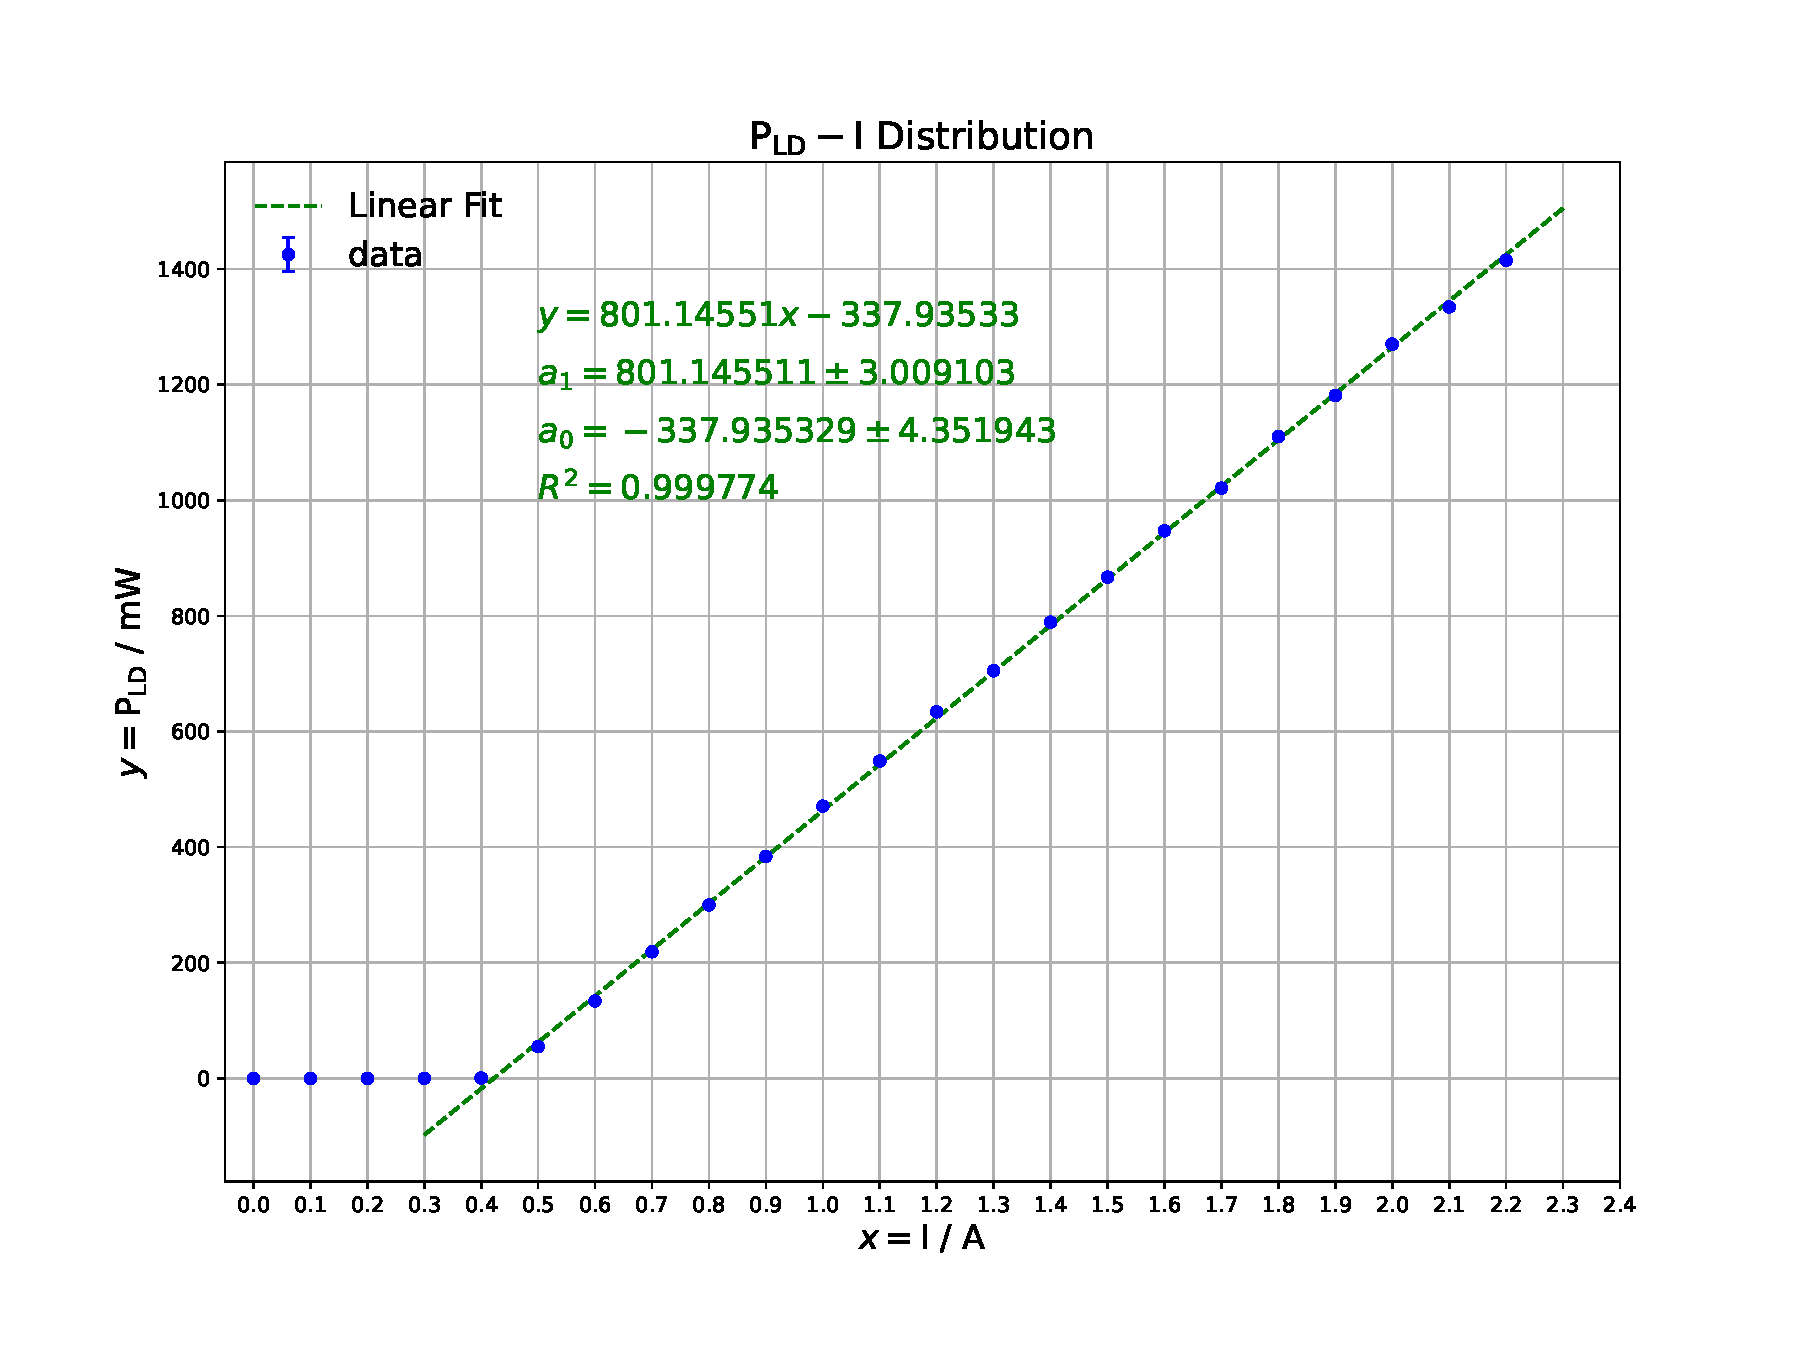
\includegraphics[height=12cm, width=16cm]{images/phyex1_fig.pdf}
 \caption{$P_{LD}-I$与超出阈值区线性拟合分布图}
 \label{fig:fig1}
\end{figure}\\
这里通过线性回归,我们可以算出阈值电流
\begin{equation}
\rm I_{th}=a_1/|a_0|=0.422A
\end{equation}
考虑到误差传递,则有
\begin{equation}
\rm \sigma_{I_{th}}=I_{th}*\sqrt{(\frac{\sigma_{a_1}}{a_1})^2+(\frac{\sigma_{a_0}}{a_0})^2}=0.006A\\
\end{equation}
因此阈值电流测量结果为
\begin{equation}
\rm I_{th}\pm\sigma_{I_{th}}=(0.422\pm0.006)A
\end{equation}
\begin{comment}
如果需要索引参考文献,请使用\cite{Erdos01}, 同时已经将参考文献的项目模版在文末写出。
\end{comment}
%%%%%%%%%%%%%%%%%%%%%%%%%%%%%%%%%%%%%%%%%%%%%%%%%%%%%%%%%%%%%%%%%%%%%%%%%%%%%%%%%%%%%%%%%%
\newpage
\subsection{$\mathrm{P_{IR} - I}$分布}\label{sub:ctl}
分别使用$\rm Nd:YVO_4$和$\rm Nd:YAG$激光晶体,测量其在最佳工作状态下,激光功率$P_{IR}$随泵浦电流I的变化,并获得固体激光器的转换效率$\eta = p_{IR}/P_{LD}$.
\subsubsection{$\rm{Nd:YVO_4}$晶体条件}
$\rm Nd:YVO_4$激光晶体的测量结果如下图\ref{fig:fig2}. 
\begin{figure}[ht]
 \centering
 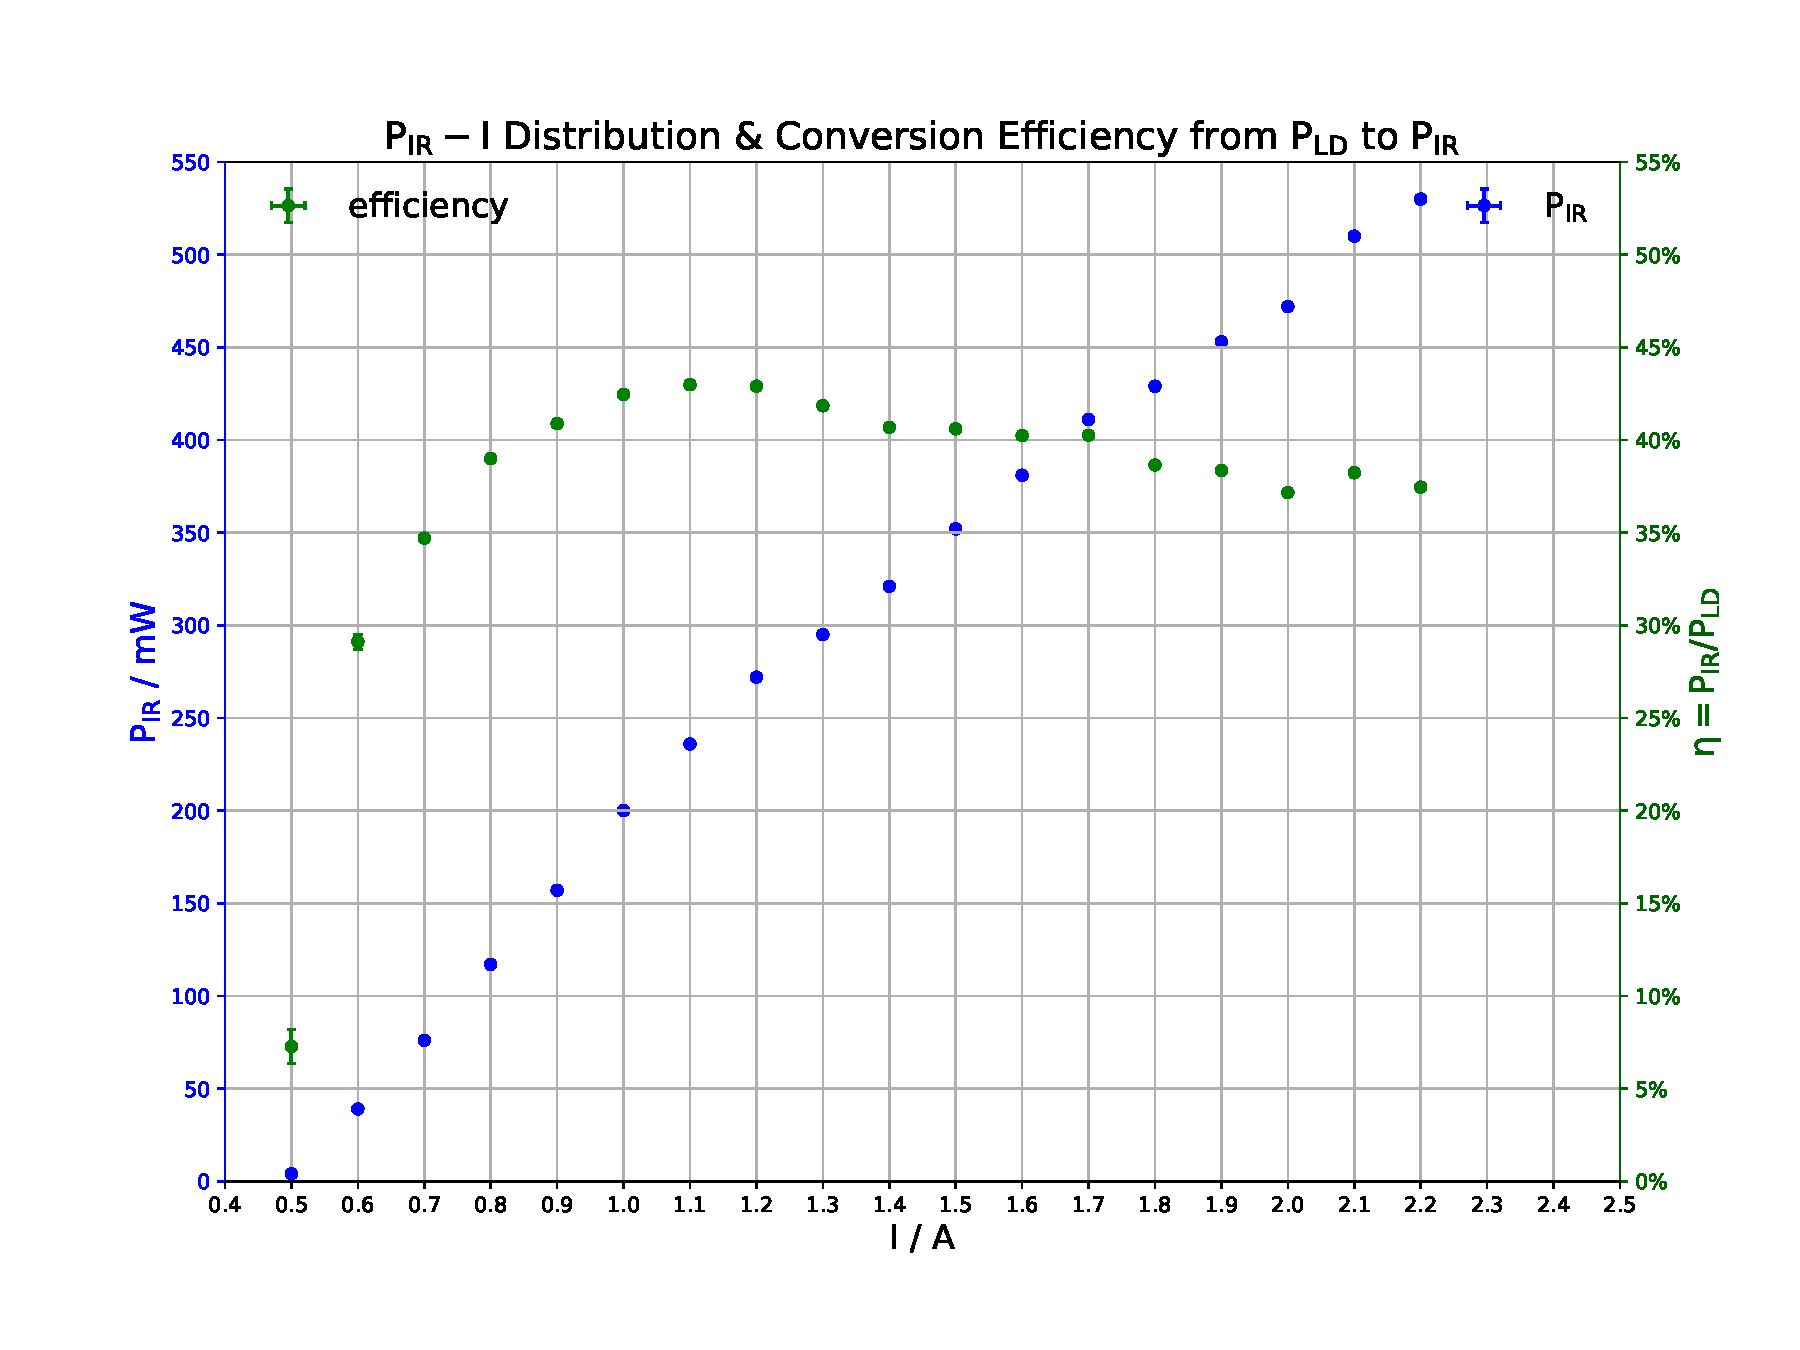
\includegraphics[height=12cm, width=16cm]{images/phyex2_fig.pdf}
 \caption{$\rm{Nd:YVO_4}$晶体条件下$P_{IR}-I$与激光器转化效率分布图}
 \label{fig:fig2}
\end{figure}\\
我们可以看到在阈值电流以上,激光功率$P_{IR}$随泵浦电流I近乎直线增长, 而固体激光器的转换效率在测量区域内最高接近$45\%$, 平均约为$40\%$
\newpage
\subsubsection{$\rm{Nd:YAG}$晶体条件}
$\rm Nd:YAG$激光晶体的测量结果如下图\ref{fig:fig3}. 
\begin{figure}[ht]
 \centering
 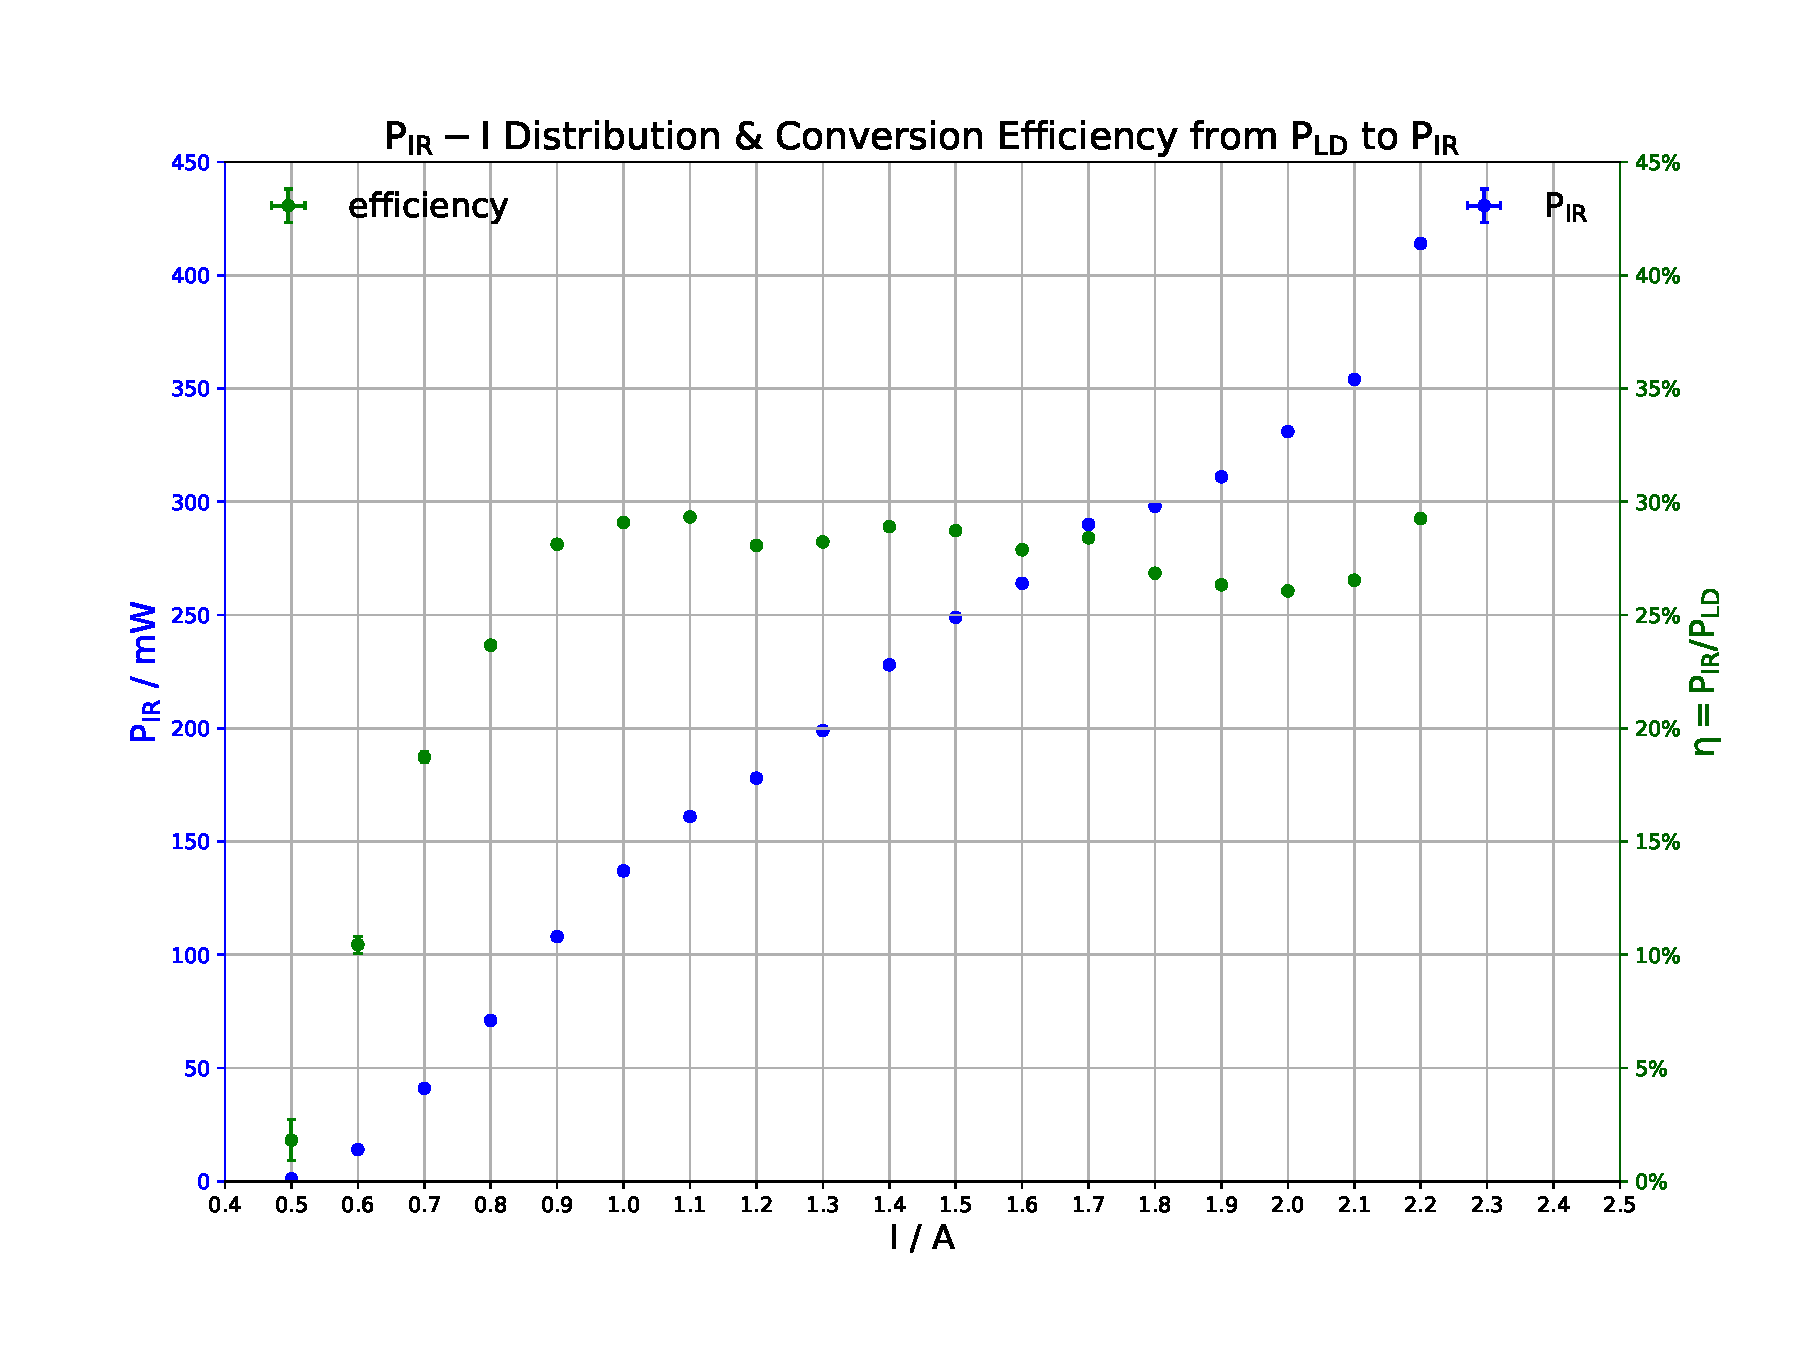
\includegraphics[height=12cm, width=16cm]{images/phyex3_fig.pdf}
 \caption{$\rm{Nd:YAG}$晶体条件下$P_{IR}-I$与激光器转化效率分布图}
 \label{fig:fig3}
\end{figure}\\
我们可以看到在阈值电流以上,激光功率$P_{IR}$随泵浦电流I近乎直线增长, 而固体激光器的转换效率在测量区域内最高接近$30\%$, 平均约为$25\%$

%%%%%%%%%%%%%%%%%%%%%%%%%%%%%%%%%%%%%%%%%%%%%%%%%%%%%%%%%%%%%%%%%%%%%%%%%%%%%%%%%%%%%%%%%%
\newpage
\subsection{脉冲激光功率$\rm{P_S - I}$分布}\label{sub:dat}
测量出脉冲激光的平均功率$P_S$以及脉冲激光的转换效率$\eta_{S} = p_{S}/P_{LD}$如下图\ref{fig:fig4}. 
\begin{figure}[ht]
 \centering
 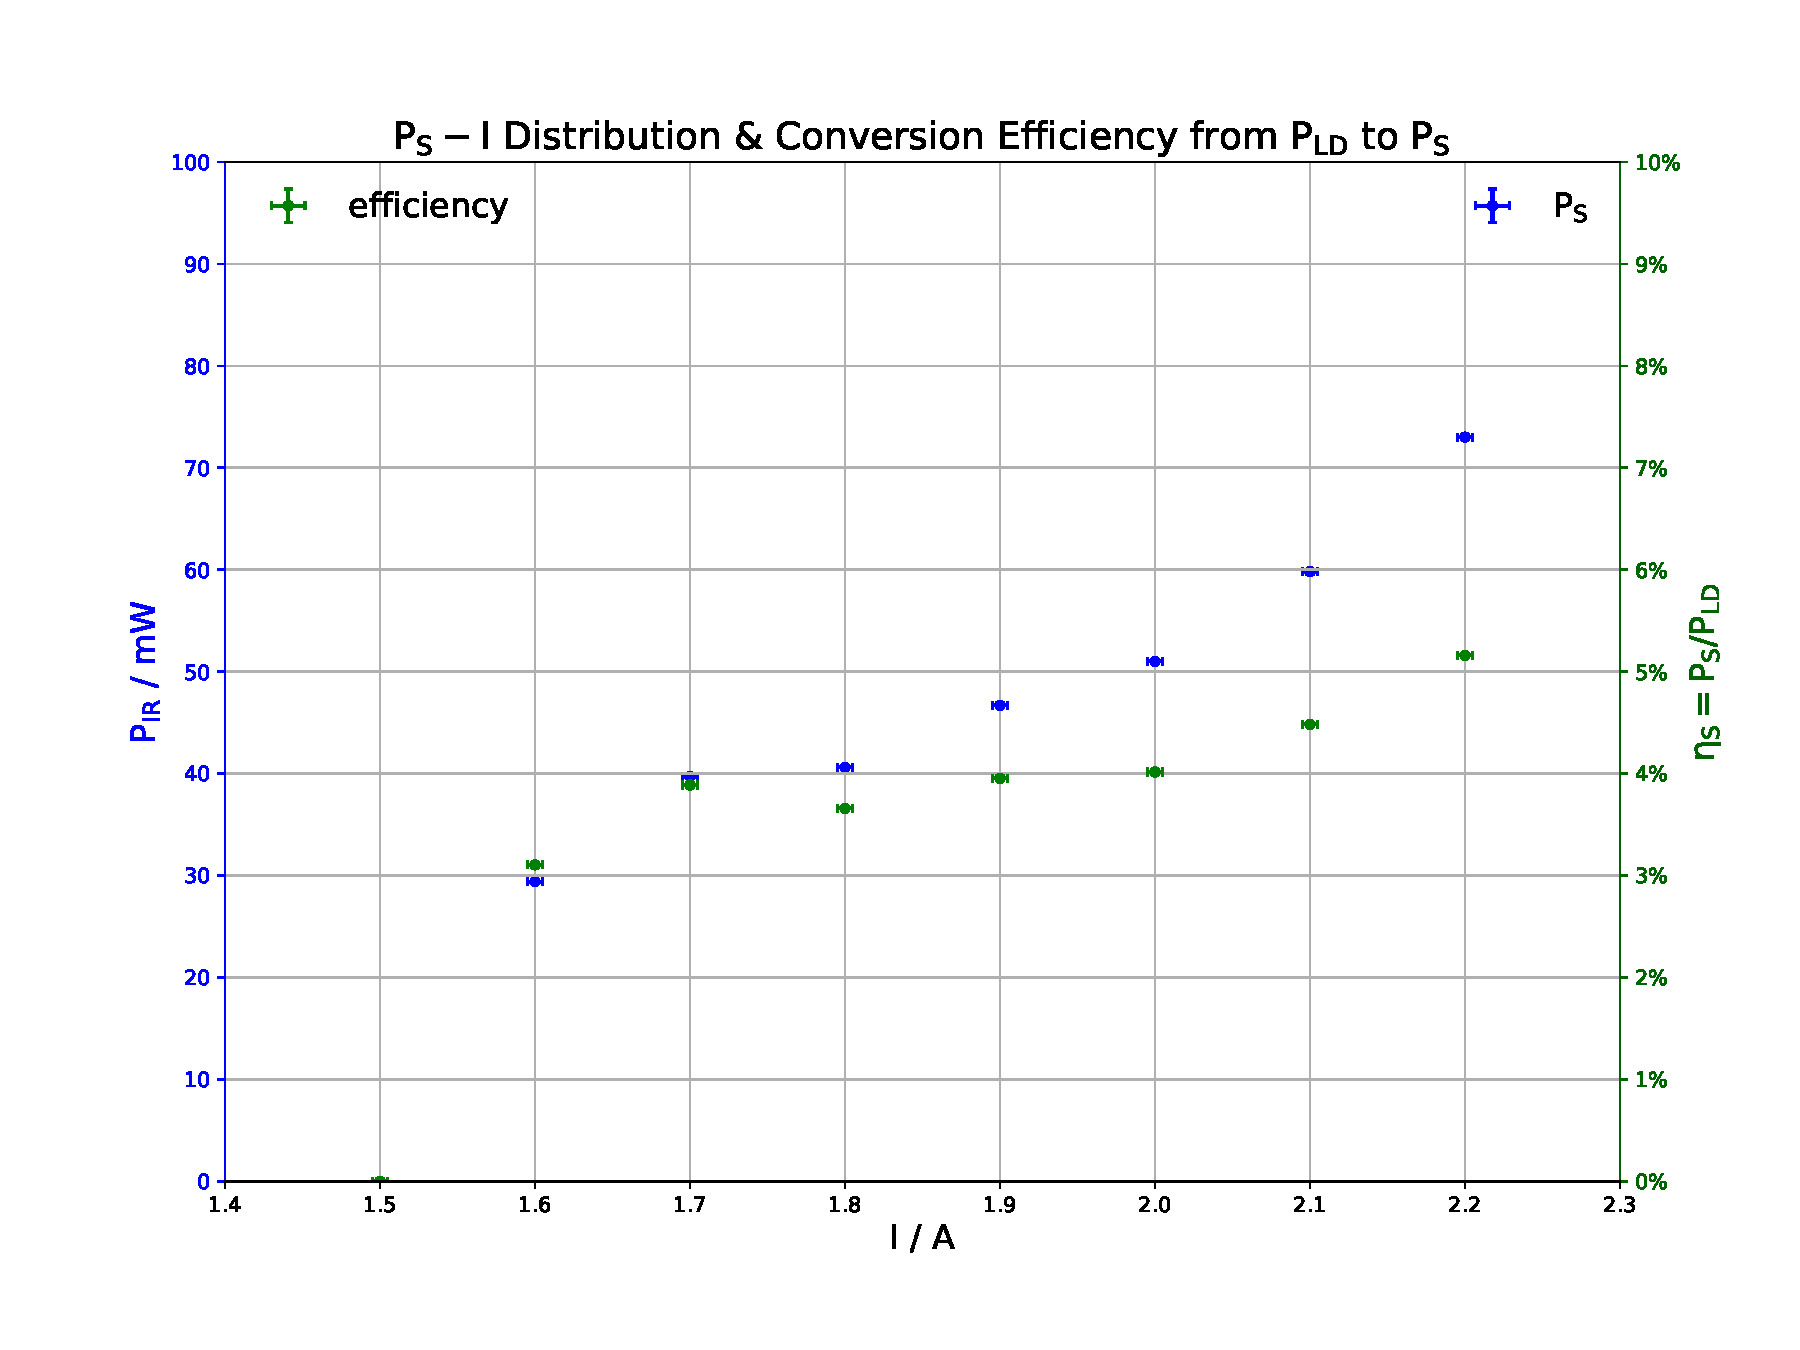
\includegraphics[height=12cm, width=16cm]{images/phyex4_fig.pdf}
 \caption{$\rm{Nd:YAG}$晶体条件下$P_{S}-I$与激光器转化效率分布图}
 \label{fig:fig4}
\end{figure}\\
我们可以看到, 在测量区域,转换效率最大刚过$5\%$, 而脉冲激光的平均功率未达到100mW
%%%%%%%%%%%%%%%%%%%%%%%%%%%%%%%%%%%%%%%%%%%%%%%%%%%%%%%%%%%%%%%%%%%%%%%%%%%%%%%%%%%%%%%%%%
\newpage
\subsection{脉冲波参数}\label{sub:pulsewave}
在示波器上观察调Q脉冲的时域特征并记录,测量出不同泵浦功率下调Q脉冲的脉宽和重复频率如下表
\begin{table}[htp]
\caption{不同泵浦功率下调Q脉冲的脉宽和重复频率}\label{tab:signaldef}
\begin{center}
	\begin{tabular}{|l|l|l|p{6cm}|}
	\hline
	\textbf{泵浦电流$\rm I/A$} &\textbf{泵浦功率$\rm $P_{LD}/mW$} & \textbf{脉冲半高宽$\rm \tau /ns$} & \textbf{重复频率$\rm f/kHz$}\\ \hline \hline
	$1.80$  & $1110$    & $69.00$ 	& $2.41$ \\ \hline
	$2.00$ 	& $1270$    & $67.00$   & $2.91$ \\ \hline
	$2.20$  & $1415$    & $69.00$   & $4.29$ \\ \hline
	\hline
	\end{tabular}
\end{center}
\end{table}\\
可以看出脉冲半高宽基本不随泵浦电流I(也就是泵浦功率$P_{LD}$)变化,而重复频率随泵浦电流I上升而急剧上升
%%%%%%%%%%%%%%%%%%%%%%%%%%%%%%%%%%%%%%%%%%%%%%%%%%%%%%%%%%%%%%%%%%%%%%%%%%%%%%%%%%%%%%%%%%
\subsection{$\rm{P_{2\omega} - I}$分布}\label{sub:doublefrequency}
测量得到二倍频激光的功率和转换效率如下图\ref{fig:fig5}. 
\begin{figure}[ht]
 \centering
 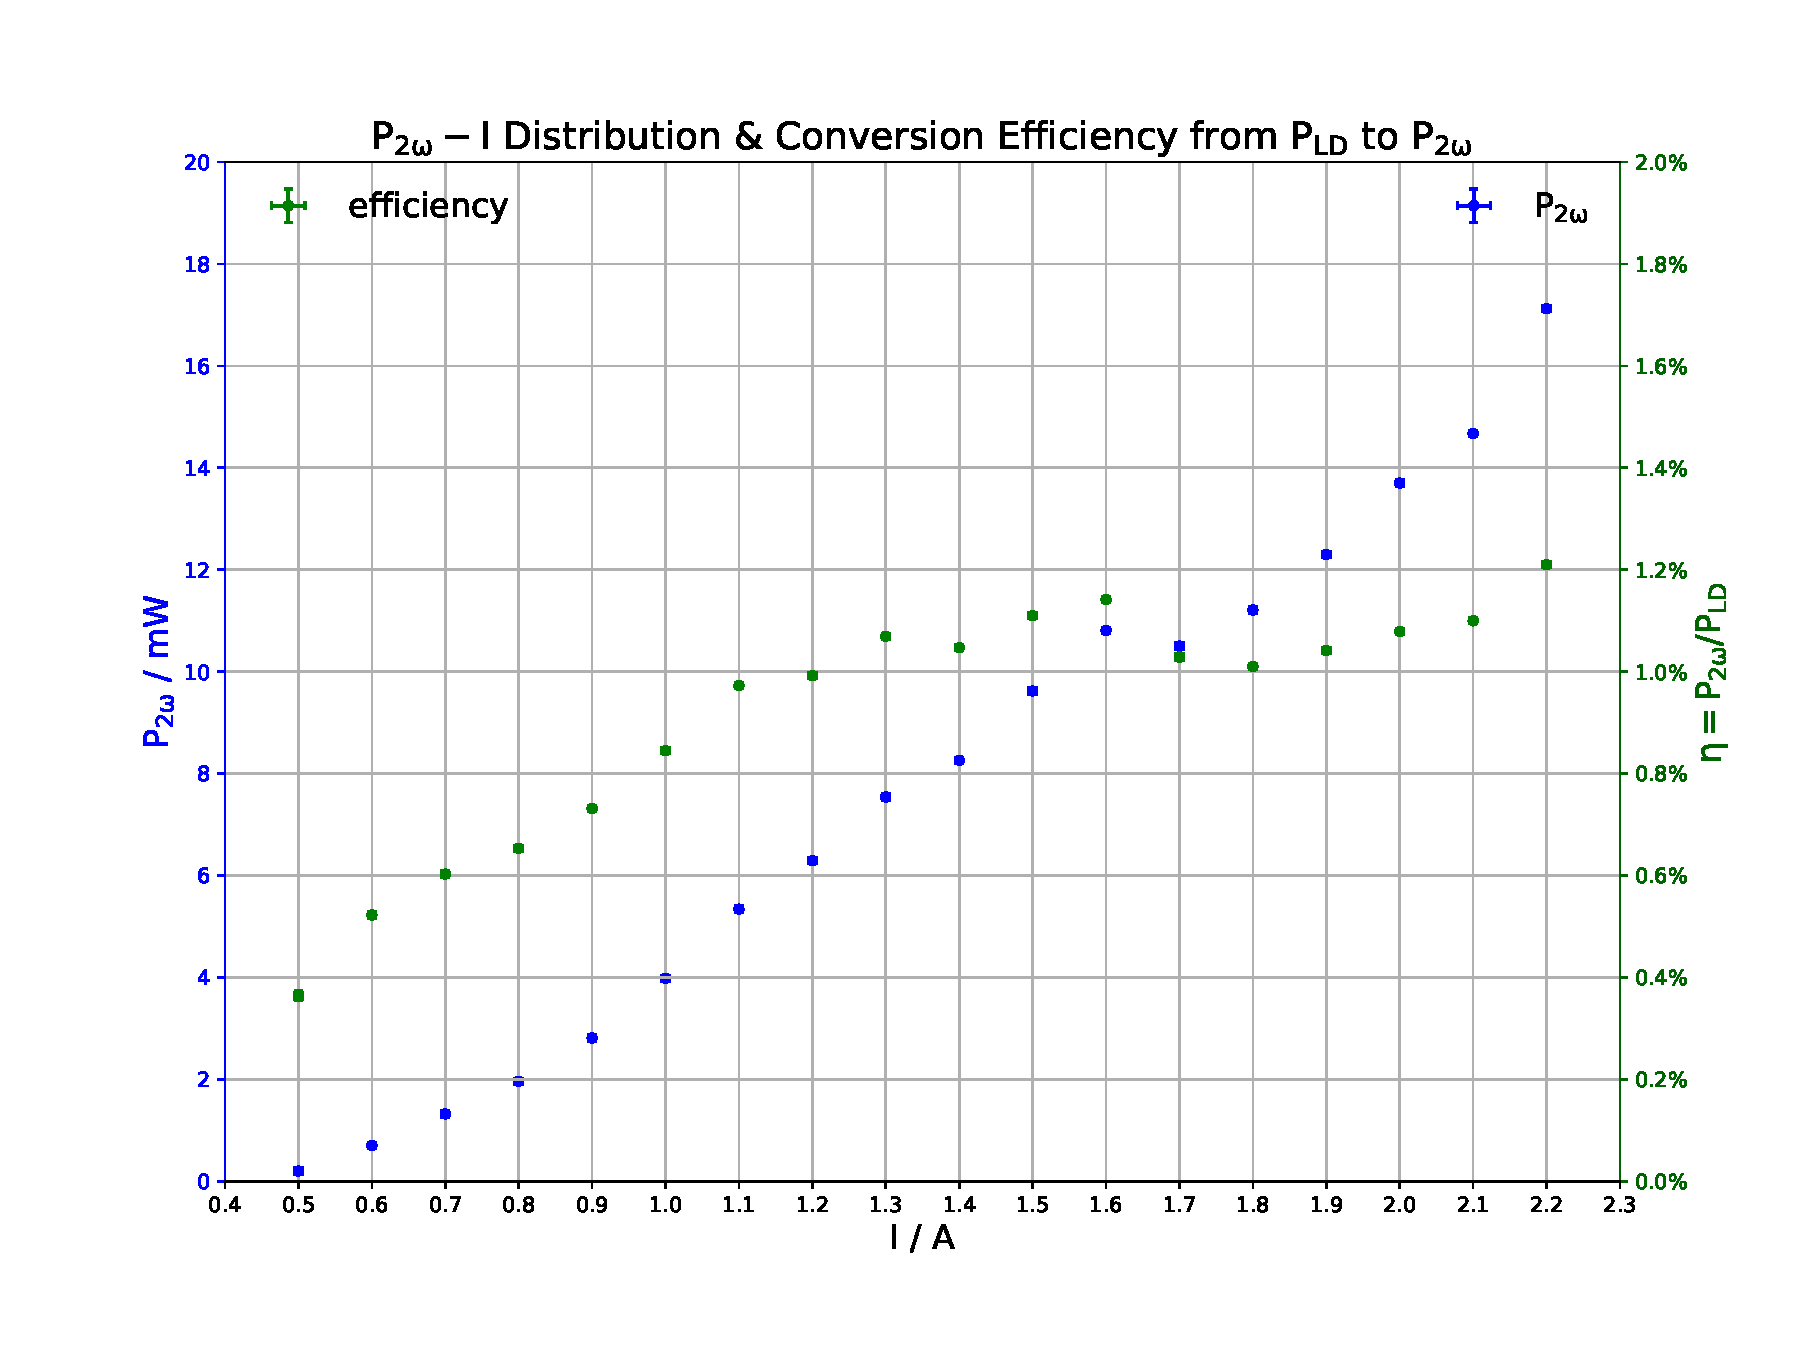
\includegraphics[height=12cm, width=16cm]{images/phyex5_fig.pdf}
 \caption{$P_{2\omega}-I$与激光器转化效率分布图}
 \label{fig:fig5}
\end{figure}\\
可以看到转化效率在$1\%$附近,极低.

%add more subsections for other block

% -----------------------------------Conclusion----------------------------------------
\newpage
\section{结论}\label{conclusions}
结论基本已经在上一节给出,此处不再赘述.\\

% -----------------------------------Acknowledgements----------------------------------------

\section{致谢}\label{acknowledgments}
感谢同组同学在实验中的辛勤工作,以及蒋老师的悉心指导.

% -----------------------------------Questions----------------------------------------
\begin{comment}
\newpage
\section{思考题}\label{questions}
实际上我一个都回答不出来,所以我把这部分注释掉了
\end{comment}

\begin{comment}
% -----------------------------------Appendix----------------------------------------
\appendix
\section{代码}\label{sub:app.code}
请在附录\ref{sub:app.code}中添加代码。请使用如下Scala的语法高亮描述方法。
\begin{scala}
class TopIO extends Bundle() {
	val boot = Input(Bool()) 
// imem and dmem interface for Tests
	val test_im_wr		= Input(Bool())
	val test_im_rd 		= Input(Bool())
	val test_im_addr 	= Input(UInt(32.W))
	val test_im_in 		= Input(UInt(32.W))
	val test_im_out 	= Output(UInt(32.W))

	val test_dm_wr		= Input(Bool())
	val test_dm_rd 		= Input(Bool())
	val test_dm_addr 	= Input(UInt(32.W))
	val test_dm_in 		= Input(UInt(32.W))
	val test_dm_out 	= Output(UInt(32.W))

	val valid			= Output(Bool())
}
class Top extends Module() {
	val io 		= IO(new TopIO())//in chisel3, io must be wrapped in IO(...) 
	//...
	when (io.boot & io.test_im_wr){
		imm(io.test_im_addr) := io.test_im_in
		} .elsewhen (io.boot & io.test_dm_wr){
		// please finish it
		} //...
}
\end{scala}
\newpage
% -----------------------------------REFERENCE----------------------------------------

\begin{thebibliography}{9}

\bibitem{Erdos01} P. Erd\H os, \emph{A selection of problems and
results in combinatorics}, Recent trends in combinatorics (Matrahaza,
1995), Cambridge Univ. Press, Cambridge, 2001, pp. 1--6.

\end{thebibliography}
\end{comment}
\end{document}

